% Copyright 2004 by Till Tantau <tantau@users.sourceforge.net>.
%
% In principle, this file can be redistributed and/or modified under
% the terms of the GNU Public License, version 2.
%
% However, this file is supposed to be a template to be modified
% for your own needs. For this reason, if you use this file as a
% template and not specifically distribute it as part of a another
% package/program, I grant the extra permission to freely copy and
% modify this file as you see fit and even to delete this copyright
% notice. 

\documentclass{beamer}

% There are many different themes available for Beamer. A comprehensive
% list with examples is given here:
% http://deic.uab.es/~iblanes/beamer_gallery/index_by_theme.html
% You can uncomment the themes below if you would like to use a different
% one:
%\usetheme{AnnArbor}
%\usetheme{Antibes}
%\usetheme{Bergen}
%\usetheme{Berkeley}
%\usetheme{Berlin}
%\usetheme{Boadilla}
%\usetheme{boxes}
%\usetheme{CambridgeUS}
%\usetheme{Copenhagen}
%\usetheme{Darmstadt}
%\usetheme{default}
%\usetheme{Frankfurt}
%\usetheme{Goettingen}
%\usetheme{Hannover}
%\usetheme{Ilmenau}
%\usetheme{JuanLesPins}
%\usetheme{Luebeck}
\usetheme{Madrid}
%\usetheme{Malmoe}
%\usetheme{Marburg}
%\usetheme{Montpellier}
%\usetheme{PaloAlto}
%\usetheme{Pittsburgh}
%\usetheme{Rochester}
%\usetheme{Singapore}
%\usetheme{Szeged}
%\usetheme{Warsaw}

\usepackage{media9}
\usepackage{textpos}

%\setbeamerfont{footline}{size=\fontsize{9}{11}\selectfont}

\title [Developing SPH Based Modeling of Plume] {Developing SPH Based Modeling of Volcanic Plumes using Modified SPH Schemes}

% A subtitle is optional and this may be deleted
%\subtitle{Optional Subtitle}

\author [Z. Cao, A. Patra] {
    Zhixuan Cao\inst{1} \and
    Abani Patra\inst{1,2}
    }
% - Give the names in the same order as the appear in the paper.
% - Use the \inst{?} command only if the authors have different
%   affiliation.
%\institute[Universities of Somewhere and Elsewhere] % (optional, but mostly needed)
%{
%  \inst{1}%
%  Department of Computer Science\\
%  University of Somewhere
%  \and
%  \inst{2}%
%  Department of Theoretical Philosophy\\
%  University of Elsewhere}
  
\institute [UB]{
\inst{1}
Department of Mechanical and Aerospace \\
University at Buffalo, Buffalo, New York, U.S.A.
\and
\inst{2}
Center for Computational Research \\
University at Buffalo, Buffalo, New York, U.S.A.
%\and
%\inst{2}
%Computational, Data Sciences \& Eng.,\\
%University at Buffalo, Buffalo, New York, U.S.A.
 }
% - Use the \inst command only if there are several affiliations.
% - Keep it simple, no one is interested in your street address.

\date [14th USNCCM] {14th U.S. National Congress on Computational Mechanics}
% - Either use conference name or its abbreviation.
% - Not really informative to the audience, more for people (including
%   yourself) who are reading the slides online

\subject {Numerical modelling}
% This is only inserted into the PDF information catalog. Can be left
% out. 

% If you have a file called "university-logo-filename.xxx", where xxx
% is a graphic format that can be processed by latex or pdflatex,
% resp., then you can add a logo as follows:

%\pgfdeclareimage[height=0.5cm]{university-logo}{UB_Stacked_SUNY} \logo{\pgfuseimage{university-logo}}

% Delete this, if you do not want the table of contents to pop up at
% the beginning of each subsection:
\AtBeginSection[]
{
  \begin{frame}<beamer>{Outline}
    \tableofcontents[currentsection]
  \end{frame}
}

% Let's get started
\begin{document}

\begin{frame}
  \titlepage
\end{frame}

\addtobeamertemplate{frametitle}{}{%
\begin{textblock*}{350mm}(.80\textwidth,-0.85cm)

\includegraphics[height=0.75cm,width=2.5cm]{UB_Secondary_SUNY_Small}
\end{textblock*}}

\begin{frame}{Outline}
  \tableofcontents
  % You might wish to add the option [pausesections]
\end{frame}
%-----------------------------------------------------
% Section and subsections will appear in the presentation overview
% and table of contents.
%----------------------------------------------------------------------------
\section{Motivation for Choosing SPH}
\begin{frame}{Motivation for Choosing SPH}
 Volcanic plume development is essentially a multi-phase, turbulent mixing process coupled with heat transfer and other microphysics processes without pre-defined boundaries. SPH (Smoothed particle hydrodynamics), as a mesh-less method, is suitable for such problems for several reasons:
  \begin{itemize}
  \item {
    SPH is able to automatically construct the interface.
  }
  \item {
    Multiphase modeling is easily accomplished using SPH 
  }
  \item {
    Adding of new physics and new phases is easier in terms of programming in SPH 
  }
  \item {
    With very limited global communication requirements, SPH solvers can scale better for parallel computing than grid based ones.
  }
  \end{itemize}
\end{frame}
%---------------------------------------------------------------------------
\section{Physics Model}
\begin{frame}{Governing Equations}
\noindent
\begin{minipage}{.505\textwidth}
The governing equations and EOS for closing the system of equations:
\begin{equation}
\dfrac{\partial \rho}{\partial t} + \nabla \cdot \left(\rho \textbf{v}\right) = 0 \label{eq:gov-cs-rho}
\end{equation}
\begin{equation}
\dfrac{\partial \rho \xi}{\partial t} + \nabla \cdot \left(\rho \xi \textbf{v}\right) = 0 \label{eq:gov-cs-ks}
\end{equation}
\begin{equation}
\dfrac{\partial \rho \textbf{v}}{\partial t} + \nabla \cdot \left(\rho \textbf{v} \textbf{v} + p\textbf{I}\right) = \rho \textbf{g} \label{eq:gov-cs-v} \\
\end{equation}
\begin{equation}
\dfrac{\partial \rho E}{\partial t} + \nabla \cdot \left[\left(\rho E + p \right)\textbf{v}\right] = \rho \textbf{g} \cdot\textbf{v} \label{eq:gov-cs-e}
\end{equation}
%
\begin{equation}
p = \left(\gamma_m - 1\right)\rho e \label{eq:EOS}
\end{equation}
%
\end{minipage} % This must go next to `\end{minipage}`
%
\begin{minipage}{.01\textwidth}
$\vert$\\
$\vert$\\
$\vert$\\
$\vert$\\
$\vert$\\
$\vert$\\
$\vert$\\
$\vert$\\
$\vert$\\
$\vert$\\
$\vert$\\
$\vert$\\
$\vert$\\
$\vert$\\
$\vert$\\
$\vert$\\
$\vert$\\
\end{minipage}
\begin{minipage}{.46\textwidth}
Specific heat ratio $\gamma_m$ is updated based on massfraction of erupted material:
\begin{equation}
\gamma_m = R_m/C_{vm} + 1 \label{eq:gov-gm}
\end{equation}
\begin{equation}
R_m = \xi_g R_g + \xi_a R_a  \label{eq:gov-Rm}
\end{equation}
\begin{equation}
C_{vm} = \xi_s C_{vs} + \xi_g C_{vg} + \xi_a C_{va} \label{eq:gov-Cvm}
\end{equation}
\begin{equation}
\xi_a = 1 - \xi \label{eq:gov-na}
\end{equation}
\begin{equation}
\xi_g = \xi \cdot \xi_{g0} \label{eq:gov-ng}
\end{equation}
\begin{equation}
\xi_s = \xi - \xi_g \label{eq:gov-ns}
\end{equation}
\end{minipage}
%
\end{frame}
%
\begin{frame}{Boundary Conditions}
\noindent
\begin{minipage}{.41\textwidth}
\textbf{Eruption BC}
\begin{align}
\rho =const = p/\left(R_m T\right) \label{eq:erupt_bc_rho} \\
\xi=const=1 \label{eq:erupt_bc_xi}\\
\textbf{v} = const =\{u,v,w\}^T \label{eq:erupt_bc_v}\\
\dfrac{\partial e}{\partial n}=\dot M e /\left(\pi r^2\right) \label{eq:erupt_bc_e}
\end{align} 
\textbf{No-slip wall BC}
\begin{align}
\dfrac{\partial \rho}{\partial n} = const = 0\label{eq:wall_bc_rho} \\
\dfrac{\partial \xi}{\partial n} = const = 0 \label{eq:wall_bc_xi}\\ 
\textbf{v} = const =\{0,0,0\}^T \label{eq:wall_bc_v}\\
\dfrac{\partial e }{\partial n} = 0\label{eq:wall_bc_e}
\end{align} 
\end{minipage} % This must go next to `\end{minipage}`
%
\begin{minipage}{.01\textwidth}
$\vert$\\
$\vert$\\
$\vert$\\
$\vert$\\
$\vert$\\
$\vert$\\
$\vert$\\
$\vert$\\
$\vert$\\
$\vert$\\
$\vert$\\
$\vert$\\
$\vert$\\
$\vert$\\
$\vert$\\
$\vert$\\
$\vert$\\
\end{minipage}
\begin{minipage}{.560\textwidth}
\begin{minipage}[!t]{\textwidth}
\textbf{Pressure outlet BC}
\begin{equation}
p = p_a\left(z\right)\label{eq:pressure_bc_p} 
\end{equation} 
\end{minipage}
%
\\[20mm]
%
\begin{minipage}{0.49\textwidth}
\begin{figure}[!t]
\centering
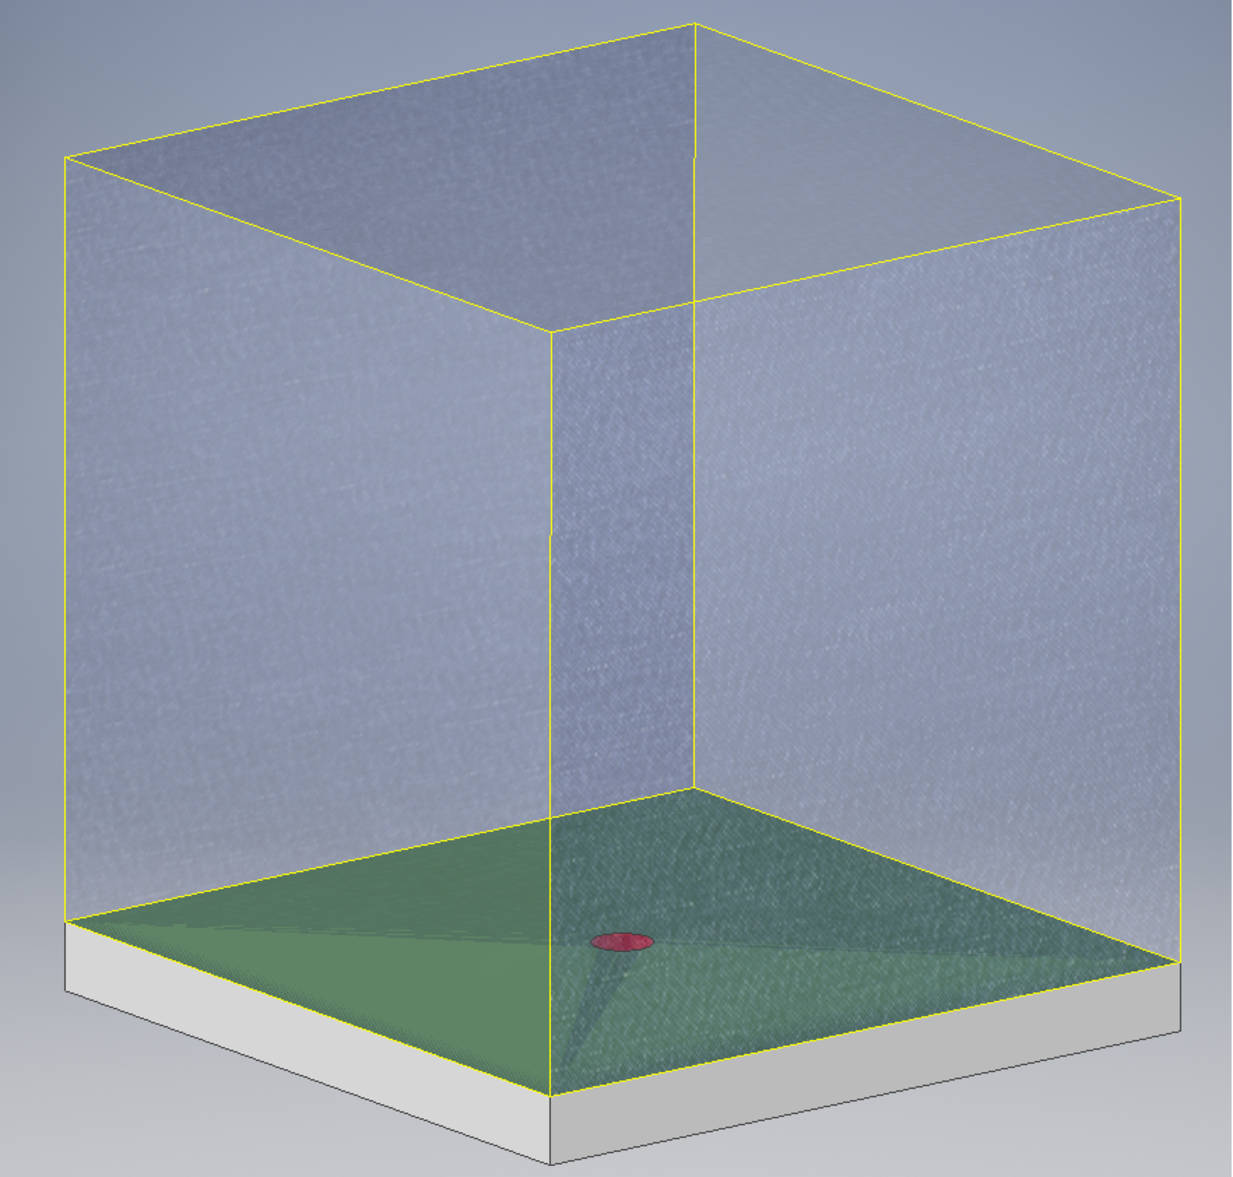
\includegraphics[width=.99\textwidth]{Domain_good}
%\caption{Scope of the problem}
\label{fig:Domain_3D}
\end{figure}
\end{minipage}
\begin{minipage}{0.49\textwidth}
\begin{figure}[!t]
\centering
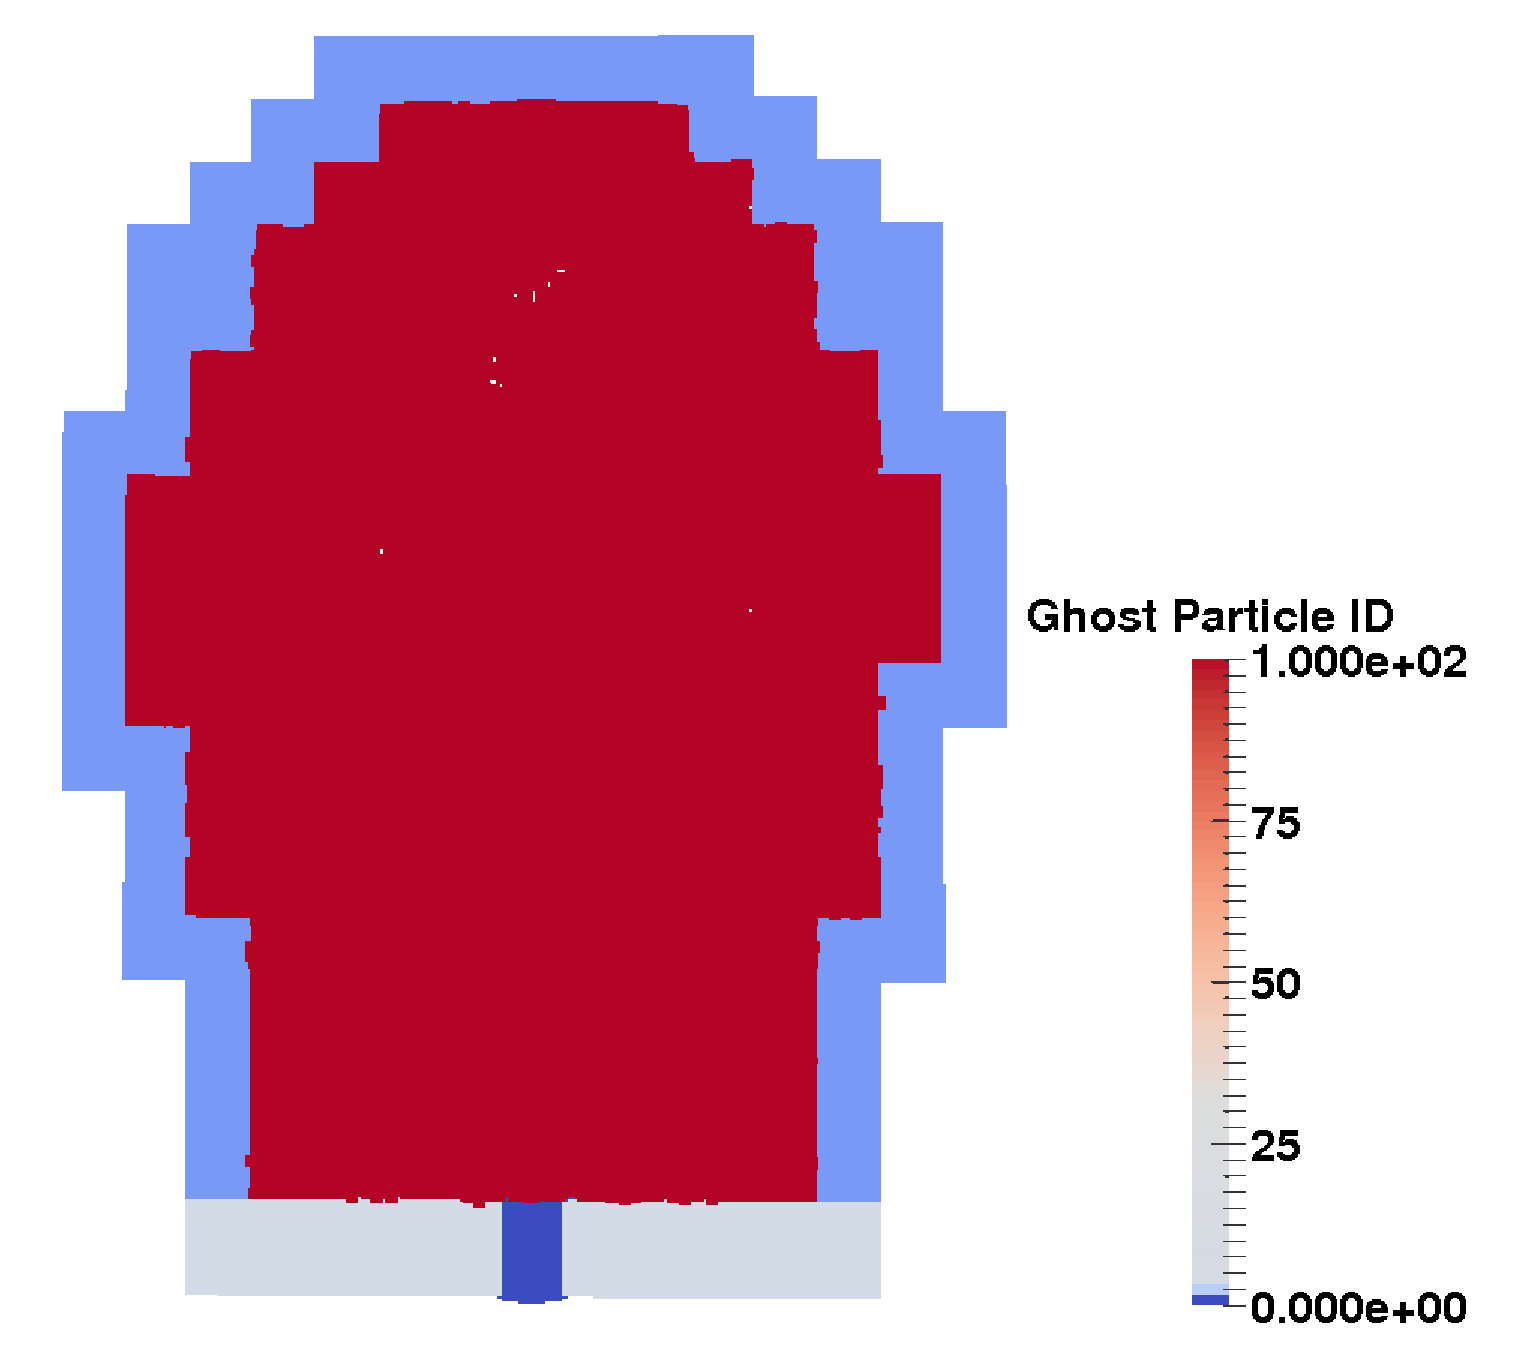
\includegraphics[width=.99\textwidth]{Boundary-condition}
%\caption{Scope of the problem}
\label{fig:BC_cut_view}
\end{figure}
\end{minipage}
%
\end{minipage}
%
\end{frame}
%--------------------------------------------------------------------
\section{SPH Discretization}
\begin{frame}{SPH Basic}
\noindent
\begin{minipage}{0.63 \textwidth}
Any function $A$ and its derivative can be approximated by:
\begin{equation}
<A\left(\textbf{x}\right)> \approx \sum_b m_b \dfrac{A_b}{\rho_b} w\left(\textbf{x}-\textbf{x}_b, h\right)
\label{eq:SPH-approximation-sum}
\end{equation}
\begin{equation}
\begin{split}
<\nabla A\left(\textbf{x}\right)> \approx \sum_b m_b \dfrac{A_b}{\rho_b} \nabla w\left(\textbf{x} - \textbf{x}_b, h\right)
\end{split} 
\label{eq:SPH-scalar-function-gradient}
\end{equation}
\end{minipage}
\begin{minipage}{0.36 \textwidth}
\begin{figure}
\center
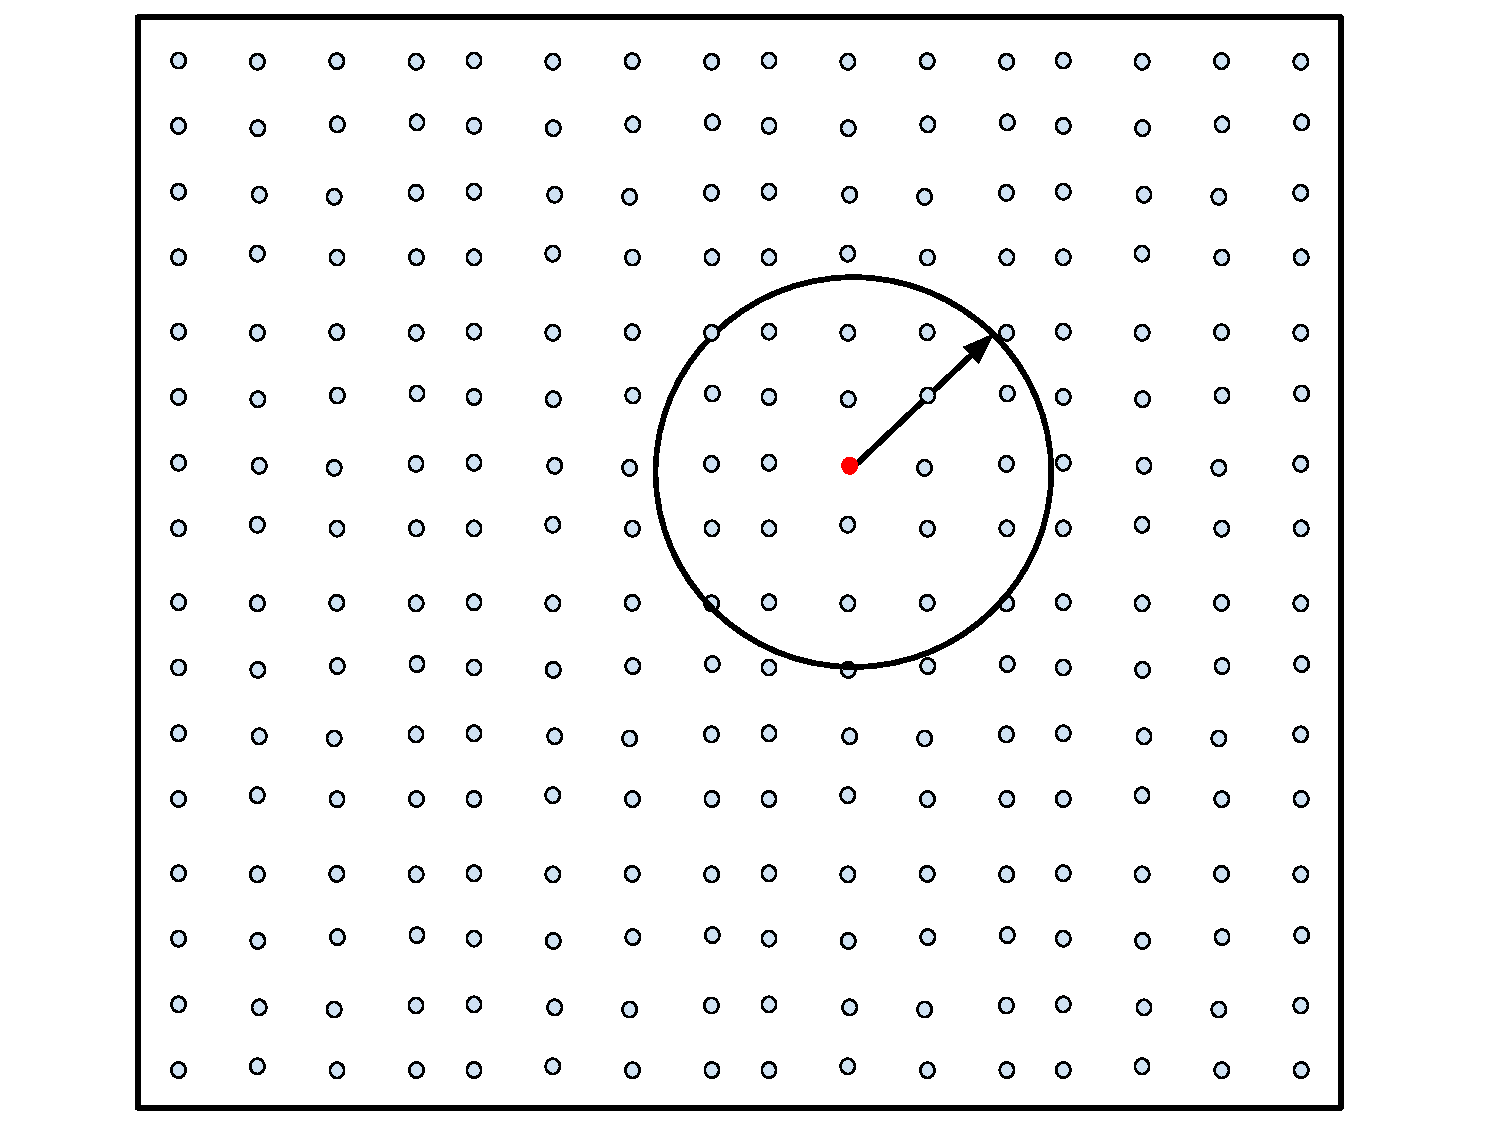
\includegraphics[width=0.99\textwidth]{Neighor-searching-noBG}
\end{figure}
\end{minipage}

Truncated Guassian kernel functions
\begin{equation}
w\left(\textbf{x} - \textbf{x}_b\right) = 
\begin{cases} 
      \dfrac{1}{\left(h \sqrt{\pi}\right)^d} exp \left[- \left(\dfrac{\textbf{x} - \textbf{x} \prime}{h} \right)^2 \right] &  \vert \textbf{x} - \textbf{x} \prime \vert \leq 3h\\
      0 & \text{Otherwise}
\end{cases}
\label{eq:SPH-kernel}
\end{equation}
\end{frame}

\begin{frame}{SPH Basic}
We adopt the following artificial viscosity developed based on Riemann Solvers,:
\begin{equation}
\Pi_{ab}^{\beta} = 
\begin{cases} 
      \dfrac{- \alpha \mu_{ab} \bar{c}_{ab} + \beta \mu_{ab}^2} {\bar{\rho}_{ab}} & \textbf{v}_{ab} \cdot \textbf{x}_{ab} < 0\\
      0 & \textbf{v}_{ab} \cdot \textbf{x}_{ab} > 0
\end{cases}
\label{eq:art-vis-shock}
\end{equation}
Where
\begin{equation}
\mu_{ab} = \dfrac{h \textbf{v}_{ab} \cdot \textbf{x}_{ab}}{\textbf{x}_{ab}^2 + \left(\eta h\right)^2} 
\end{equation}
Time step is constrained by CFL condition
\begin{equation}
\Delta t = \textrm{CFL} \min_a \bigg \lbrace \dfrac{\left[\frac{m_a}{\rho_a}\right]^{\frac{1}{d}}}{c_a} \bigg \rbrace
\end{equation}
\end{frame}

\begin{frame}{Tensile Instability and Corrected Derivatives}
The classical SPH method was known to suffer from tensile instability and boundary deficiency. To address these difficulties, we adopted a corrected SPH formulation.
\begin{equation}
A_a = \frac{\sum_b m_b \dfrac{A_b}{\rho_b} w\left(x_a-x_b, h\right)}{\sum_b m_b \dfrac{1}{\rho_b} w\left(x_a-x_b, h\right)}
\label{eq:CSP-function-approximation-1d}
\end{equation}
\begin{equation}
\nabla A_a = \frac{\sum_b m_b \dfrac{A_b - A_a}{\rho_b} \nabla_a w\left(x_a-x_b, h\right)}{\sum_b m_b \dfrac{x_b - x_a}{\rho_b} \nabla_a w\left(x_a-x_b, h\right)}
\end{equation}
\end{frame}

\begin{frame}{Multiphase SPH}
\noindent
\begin{minipage}{0.65 \textwidth}
In our model, only density needs to be updated respectively for each phase:
\begin{equation}
<\rho_{\alpha}^a>=\frac{\sum m_b w_{\alpha b} \left(h\right)}{\sum \frac{m_b}{\rho_b} w_{\alpha b} \left(h\right) +\sum \frac{m_j}{\rho_j} w_{\alpha j} \left(h\right)} \label{eq:gov-sph-d1}
\end{equation}
\begin{equation}
<\rho_\alpha^{sg}>=\frac{\sum_j m_j w_{\alpha j} \left(h\right)}{\sum \frac{m_b}{\rho_b} w_{\alpha b} \left(h\right) +\sum \frac{m_j}{\rho_j} w_{\alpha j} \left(h\right)} \label{eq:gov-sph-d2}
\end{equation}
\end{minipage}
\begin{minipage}{0.27 \textwidth}
\begin{figure}
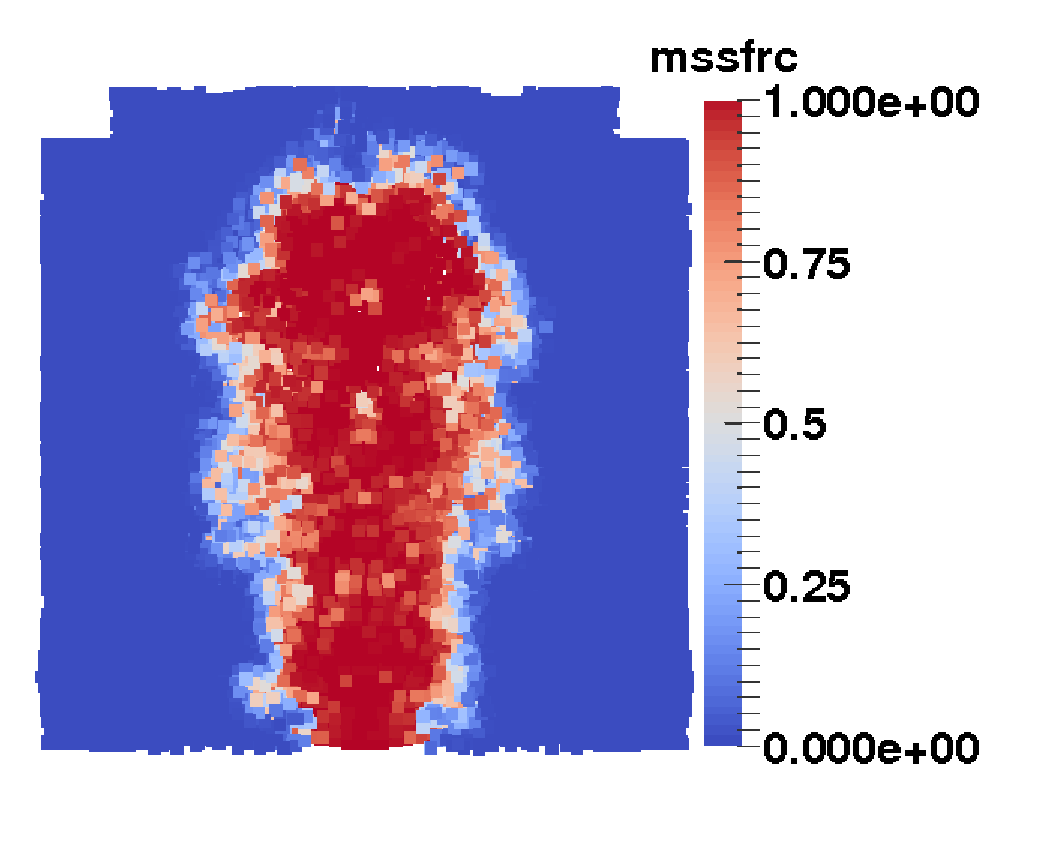
\includegraphics[width=0.95 \textwidth]{Interface_msf_rs}
\end{figure}
\begin{figure}
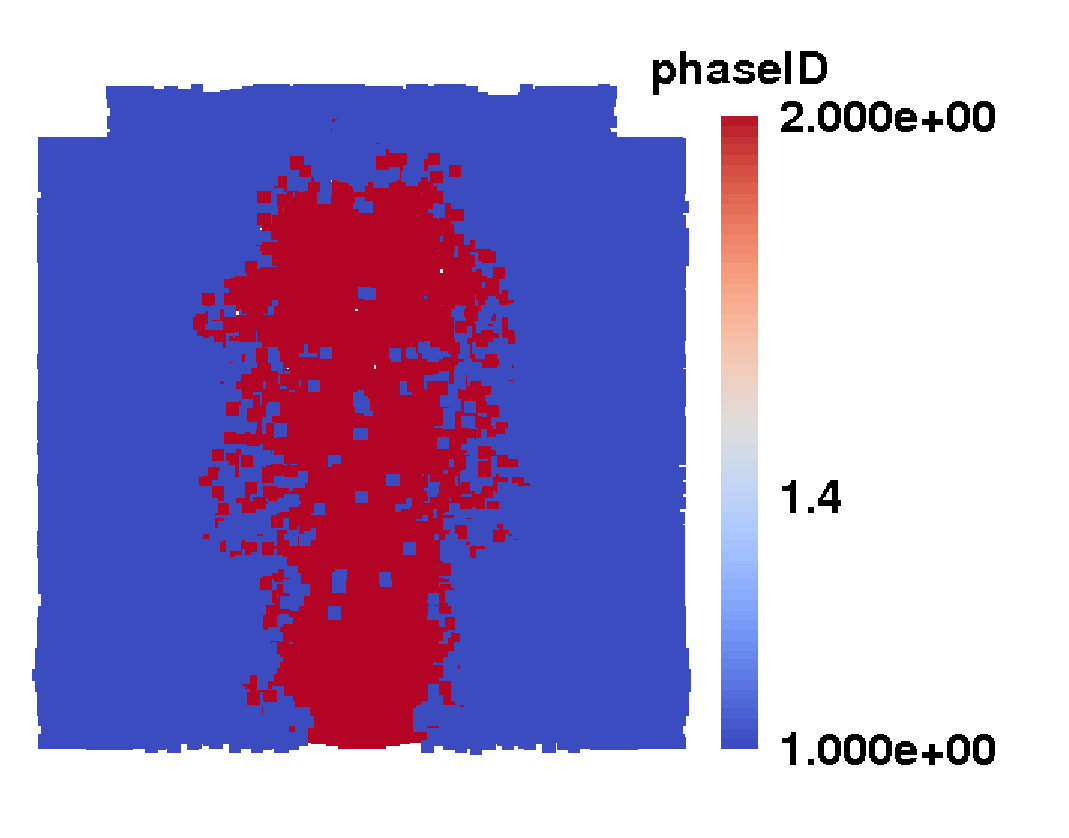
\includegraphics[width=0.95 \textwidth]{Interface_phase_rs}
\end{figure}
\end{minipage}

\begin{block}{}
  \begin{itemize}
    \item {The mass discontinuity and density discontinuity issues in traditional formulations of SPH is fixed by this new formulation
    } 
    \item {In areas far away from the interface, updating of density is exactly the same as that for single phase flow
    }
 \end{itemize}
\end{block}
\end{frame}

\begin{frame}{A LANS Type Turbulence Model}
To capture sub-particle scale momentum and energy exchange due to turbulence, we adopt a LANS type turbulence model, the $SPH-\varepsilon$ turbulence model and extend it for compressible flow.\\
Velocity is smoothed (averaged) by
\begin{equation}
\widehat{\textbf{v}}\left(\textbf{x}\right)=\int \textbf{v}\left(\textbf{x} \prime\right)G\left(\vert \textbf{x} \prime - \textbf{x} \vert, l\right) d\textbf{x} \prime
\end{equation}
Where $G$ satisfies:
\begin{equation}
\int G\left(\vert \textbf{x} \prime - \textbf{x} \vert, l\right) d\textbf{x} \prime =1
\end{equation}
\begin{equation}
\lim _{h \rightarrow 0} G\left(\textbf{x} \prime-\textbf{x}, h\right) =  \delta \left(\textbf{x} \prime - \textbf{x}\right)
\label{eq:SPH_kernel_delta}
\end{equation}
Averaging introduces an extra turbulence stress term:
\begin{equation}
\Phi_{ab}=\dfrac{\varepsilon}{2} \dfrac{\textbf{v}_{ab} \cdot \textbf{v}_{ab}}{\rho_b} \label{eq:_LANS_trub_stress}
\end{equation}
\end{frame}

\begin{frame}{Turbulent Energy Exhange}
Use Reynolds analogy to model the heat transfer due to turbulence.
\begin{equation}
\kappa=\dfrac{C_p \mu}{Pr}
\end{equation}
Instead of an analytical expression, heat transfer coeffient is calculated for each pair of particles.
\begin{equation}
\kappa_{t,ab}= 
\begin{cases} 
      0 & if \quad \textbf{v}_{ab} \cdot \textbf{x}_{ab} \leq 0 \\
      \dfrac{\varepsilon \bar{C}_{p,ab} \bar{\rho}_{ab} x_{ab}^2 \textbf{v}_{ab} \cdot \textbf{v}_{ab}}{2 S Pr_t \bar{h}_{ab} \bar{c}_{ab} \textbf{v}_{ab} \cdot \textbf{x}_{ab} } & \text{otherwise}
\end{cases}
\label{eq:SPH-LANS-heat-conductivity}
\end{equation}
\end{frame}

\begin{frame}{Discretized Governing Equations}
\begin{equation}
\begin{split}
\left\langle\dfrac{d \textbf{v}_{\alpha}}{d t}\right\rangle 
& =-\sum_b \left[ m_b \left(\dfrac{p_b}{\rho_b^2} + \dfrac{p_{\alpha}}{\rho_{\alpha}^2} + \Pi_{\alpha b}^{\beta} - \Phi_{\alpha b}\right) \bigtriangledown_{\alpha}w_{\alpha b}\left(h\right)\right] \\
& -\sum_j \left[m_j \left(\dfrac{p_j}{\rho_j^2} + \dfrac{p_{\alpha}}{\rho_{\alpha}^2} + \Pi_{\alpha j}^{\beta} - \Phi_{\alpha j}\right) \bigtriangledown_{\alpha}w_{\alpha j}\left(h\right)\right]
+\textbf{g}
\end{split}
\label{eq:gov-sph-v}
\end{equation}
\begin{equation}
\begin{split}
\left\langle\dfrac{d e_{\alpha}}{d t}\right\rangle
& = 0.5\sum_b \left[m_b \widehat{\textbf{v}_{\alpha b}}\left(\dfrac{p_b}{\rho_b^2} + \dfrac{p_{\alpha}}{\rho_{\alpha}^2} + \Pi_{\alpha b}^{\beta} - \Phi_{\alpha b}\right) \bigtriangledown_{\alpha}w_{\alpha b}\left(h\right)\right] \\
& + 2 \sum_b \dfrac{m_b}{\rho_{\alpha} \rho_b} \kappa_{t,\alpha b} \left(T_{\alpha} - T_b\right) F_{\alpha b} \left(h\right) \\
& +0.5\sum_j \left[m_j \widehat{\textbf{v}_{\alpha b}}\left(\dfrac{p_j}{\rho_j^2} + \dfrac{p_{\alpha}}{\rho_{\alpha}^2} + \Pi_{\alpha j}^{\beta} - \Phi_{\alpha j}\right) \bigtriangledown_{\alpha}w_{\alpha j}\left(h\right)\right] \\
& + 2 \sum_j \dfrac{m_j}{\rho_{\alpha} \rho_j} \kappa_{t,\alpha j} \left(T_{\alpha} - T_j\right) F_{\alpha j} \left(h\right)
\end{split}
\label{eq:gov-sph-e}
\end{equation}
\end{frame}
%------------------------------------------------------------------
\section{Verification and Validation}
\begin{frame}{Verification and Validation}
\begin{figure}
\flushleft
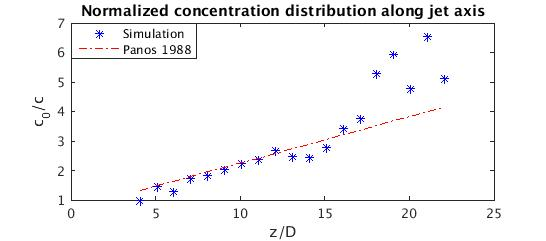
\includegraphics[width=0.245\textwidth]{../conc_along_axis}
\hfill
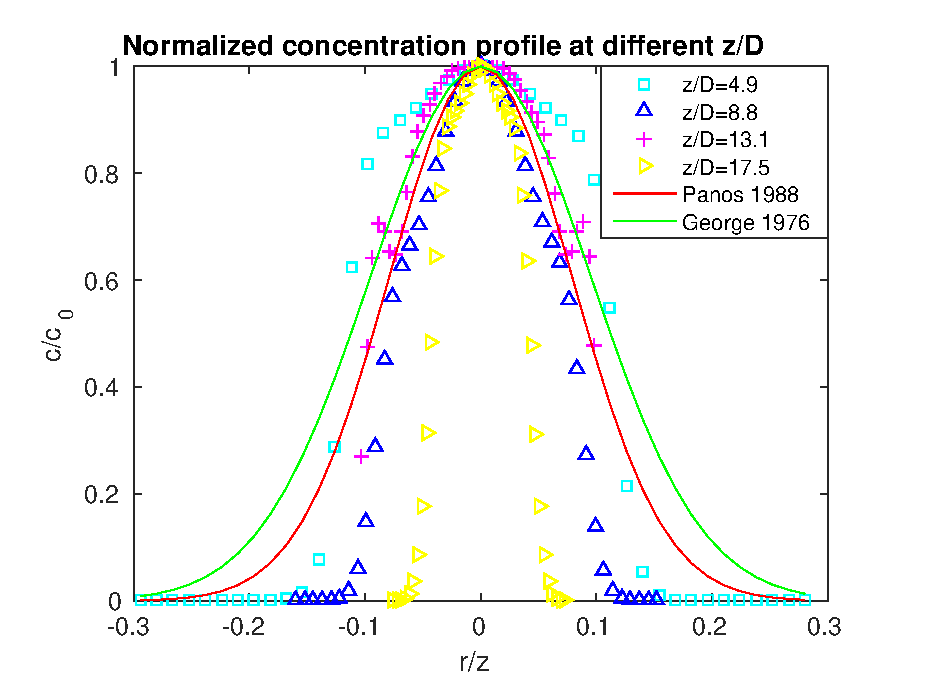
\includegraphics[width=0.245\textwidth]{../conc_cross}
\hfill
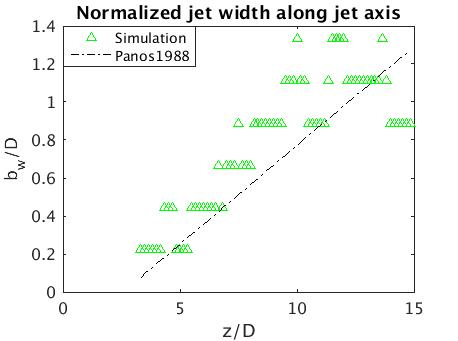
\includegraphics[width=0.245\textwidth]{../velo_along_axis}
\hfill
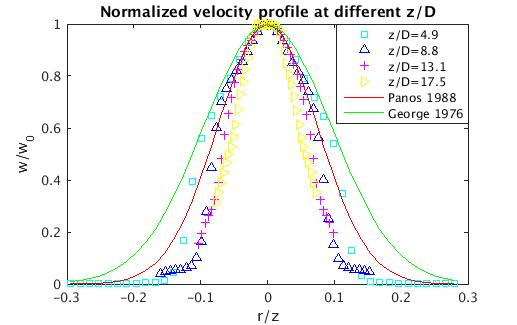
\includegraphics[width=0.245\textwidth]{../vel_cross}
\caption{JPUE test verification: dimensionless velocity and concetration distribution along centraline and across the cross-section.}
\label{fig:JPUE_all}
\end{figure}
%
\begin{figure}
\flushleft
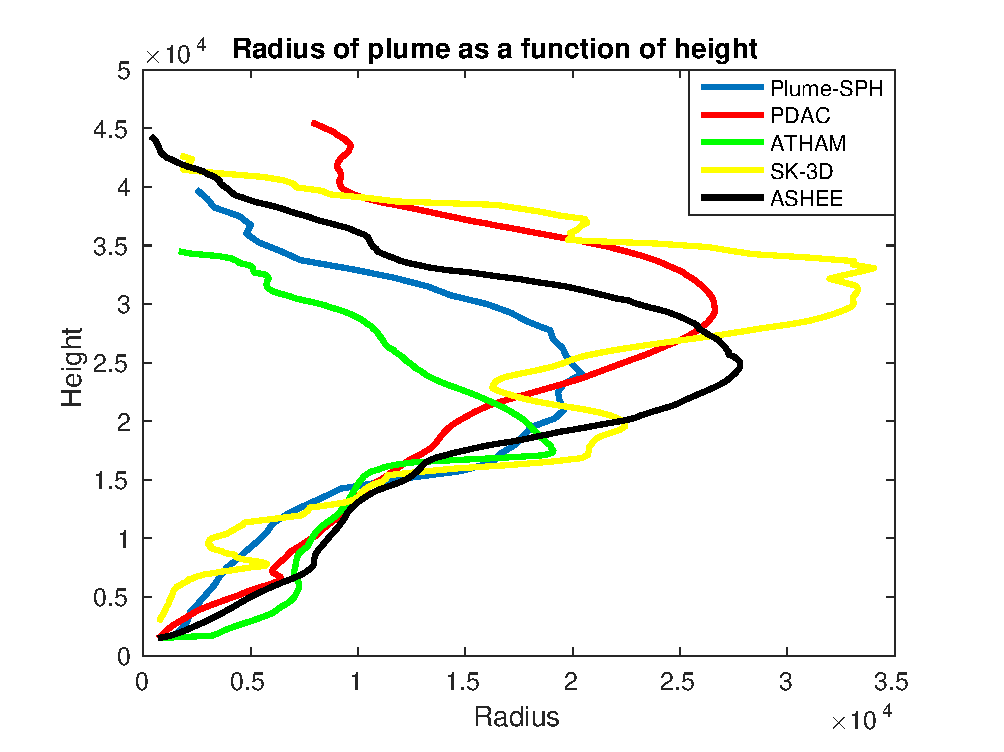
\includegraphics[width=0.245\textwidth]{../radius_strong}
\hfill
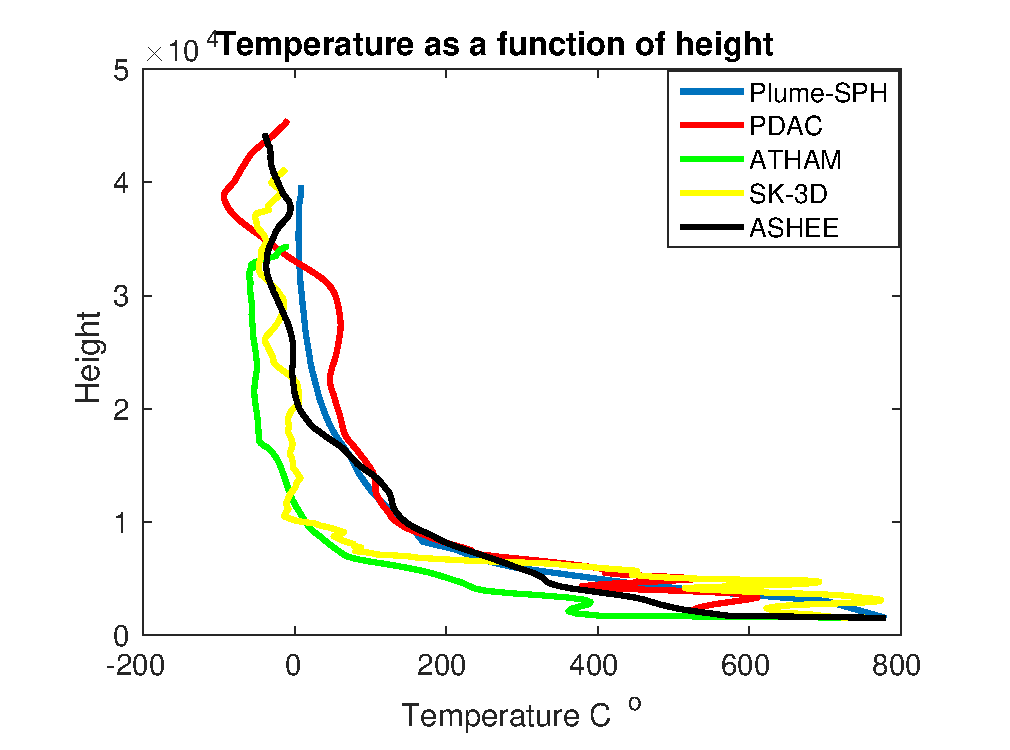
\includegraphics[width=0.245\textwidth]{../Temp}
\hfill
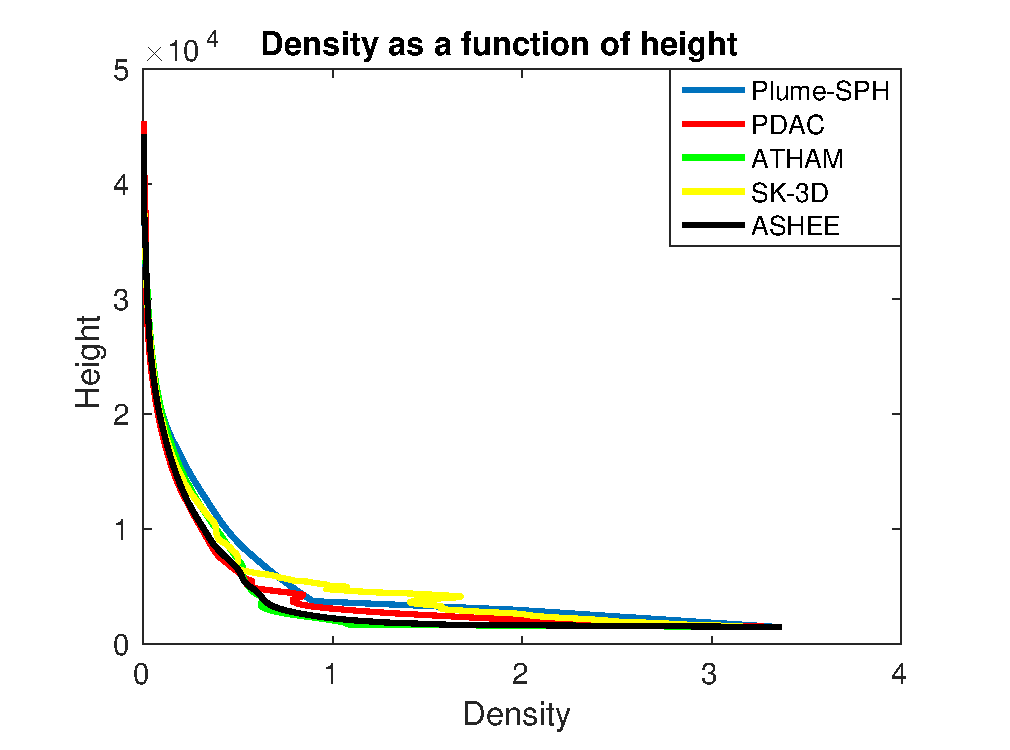
\includegraphics[width=0.245\textwidth]{../density_strong}
\hfill
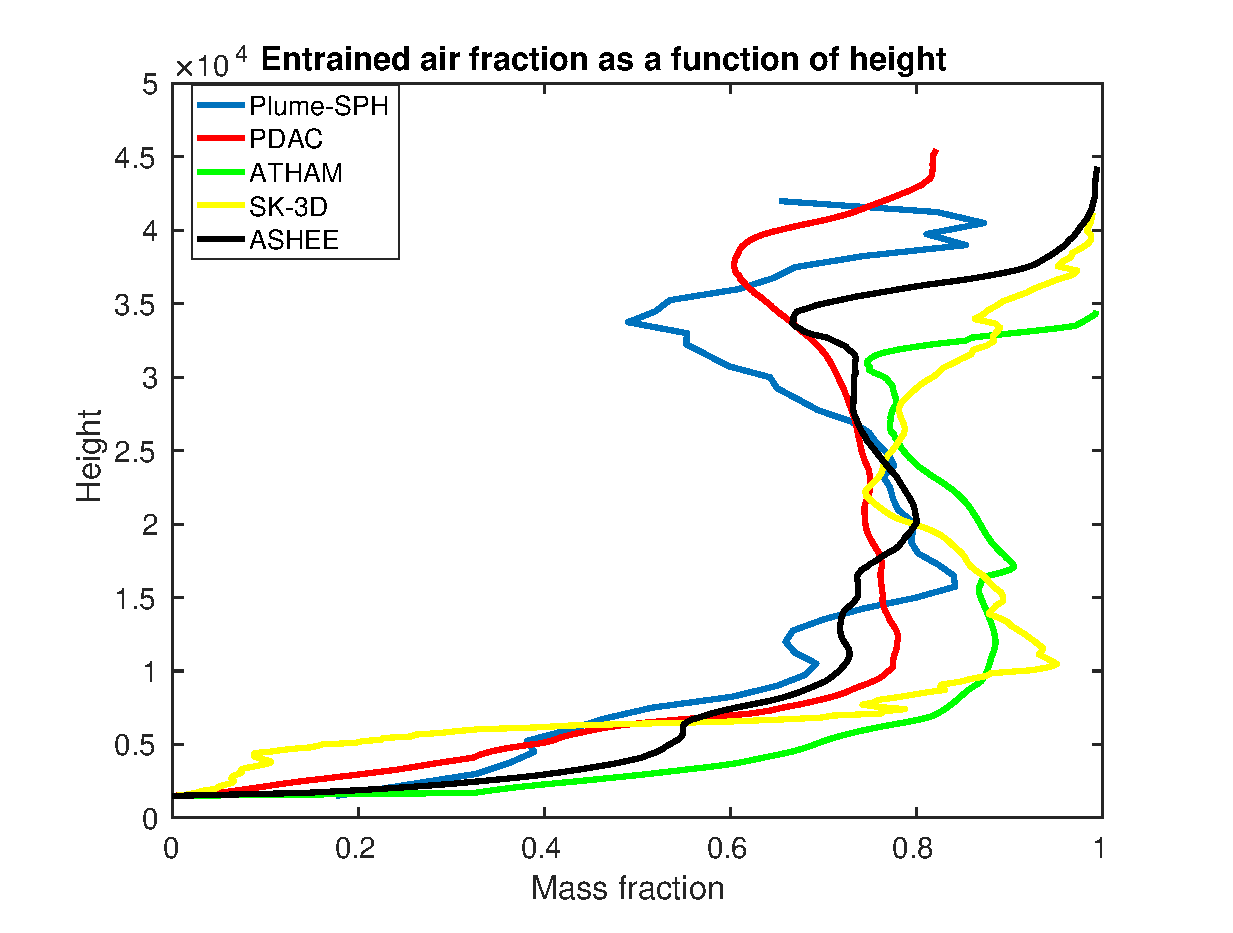
\includegraphics[width=0.245\textwidth]{mssfrc_entrained_air}
\caption{Simulation of Pinatubo (Philippines, 15 June 1991) : integrated are profiles compared with existing mesh-based models}
\label{fig:JPUE_all}
\end{figure}
\end{frame}

\begin{frame}{Annimation of Pinatubo Eruption}
Eruption condition, atmosphere, material propertities are mimic Pinatubo eruption (Philippines, 15 June 1991). \\
Eruption conditions: vent velocity is 275 $m\cdot s^{-1}$, vent gas mass fraction is 0.05, vent temperature is 1053 $K$, vent height is 1500 $km$, mass discharge rate is $1.5 \times 10^9 kg\cdot s^{-1}$. \\
%
\begin{minipage}{.32\linewidth}
\includemedia[
  label=vidA,
  width=0.99\linewidth,
  height=1.3\linewidth,
  activate=onclick,
  deactivate=onclick,
  addresource=mssfrc_sml400.mp4,
  flashvars={source=mssfrc_sml400.mp4 &loop=true}
  ]{}{VPlayer.swf}
\end{minipage}
\hfill
\begin{minipage}{.32\linewidth} 
  \includemedia[
  label=vidB,
  width=0.99\linewidth,
  height=1.3\linewidth,
  activate=onclick,
  deactivate=onclick,
  addresource=cut_view_mssfrc_sml400.mp4,
  flashvars={source=cut_view_mssfrc_sml400.mp4 &loop=true}]
  {}{VPlayer.swf}
\end{minipage}
\hfill  
\begin{minipage}{.32\linewidth} 
  \includemedia[
  label=vidC,
  width=0.99\linewidth,
  height=1.3\linewidth,
  activate=onclick,
  deactivate=onclick,
  addresource=cut_view_Involved_sml400.mp4,
  flashvars={source=cut_view_Involved_sml400.mp4 &loop=true}]
  {}{VPlayer.swf}
\end{minipage}
%  
  \mediabutton[
  mediacommand=vidA:playPause,
  mediacommand=vidB:playPause,
  mediacommand=vidC:playPause,
]{\fbox{Play/Pause}}
%
\end{frame}
%------------------------------------------------------------------
\section{Data Structure and Parallelism}
\begin{frame}{Requirement and Our Strategies}
\begin{figure}[!t]
\centering
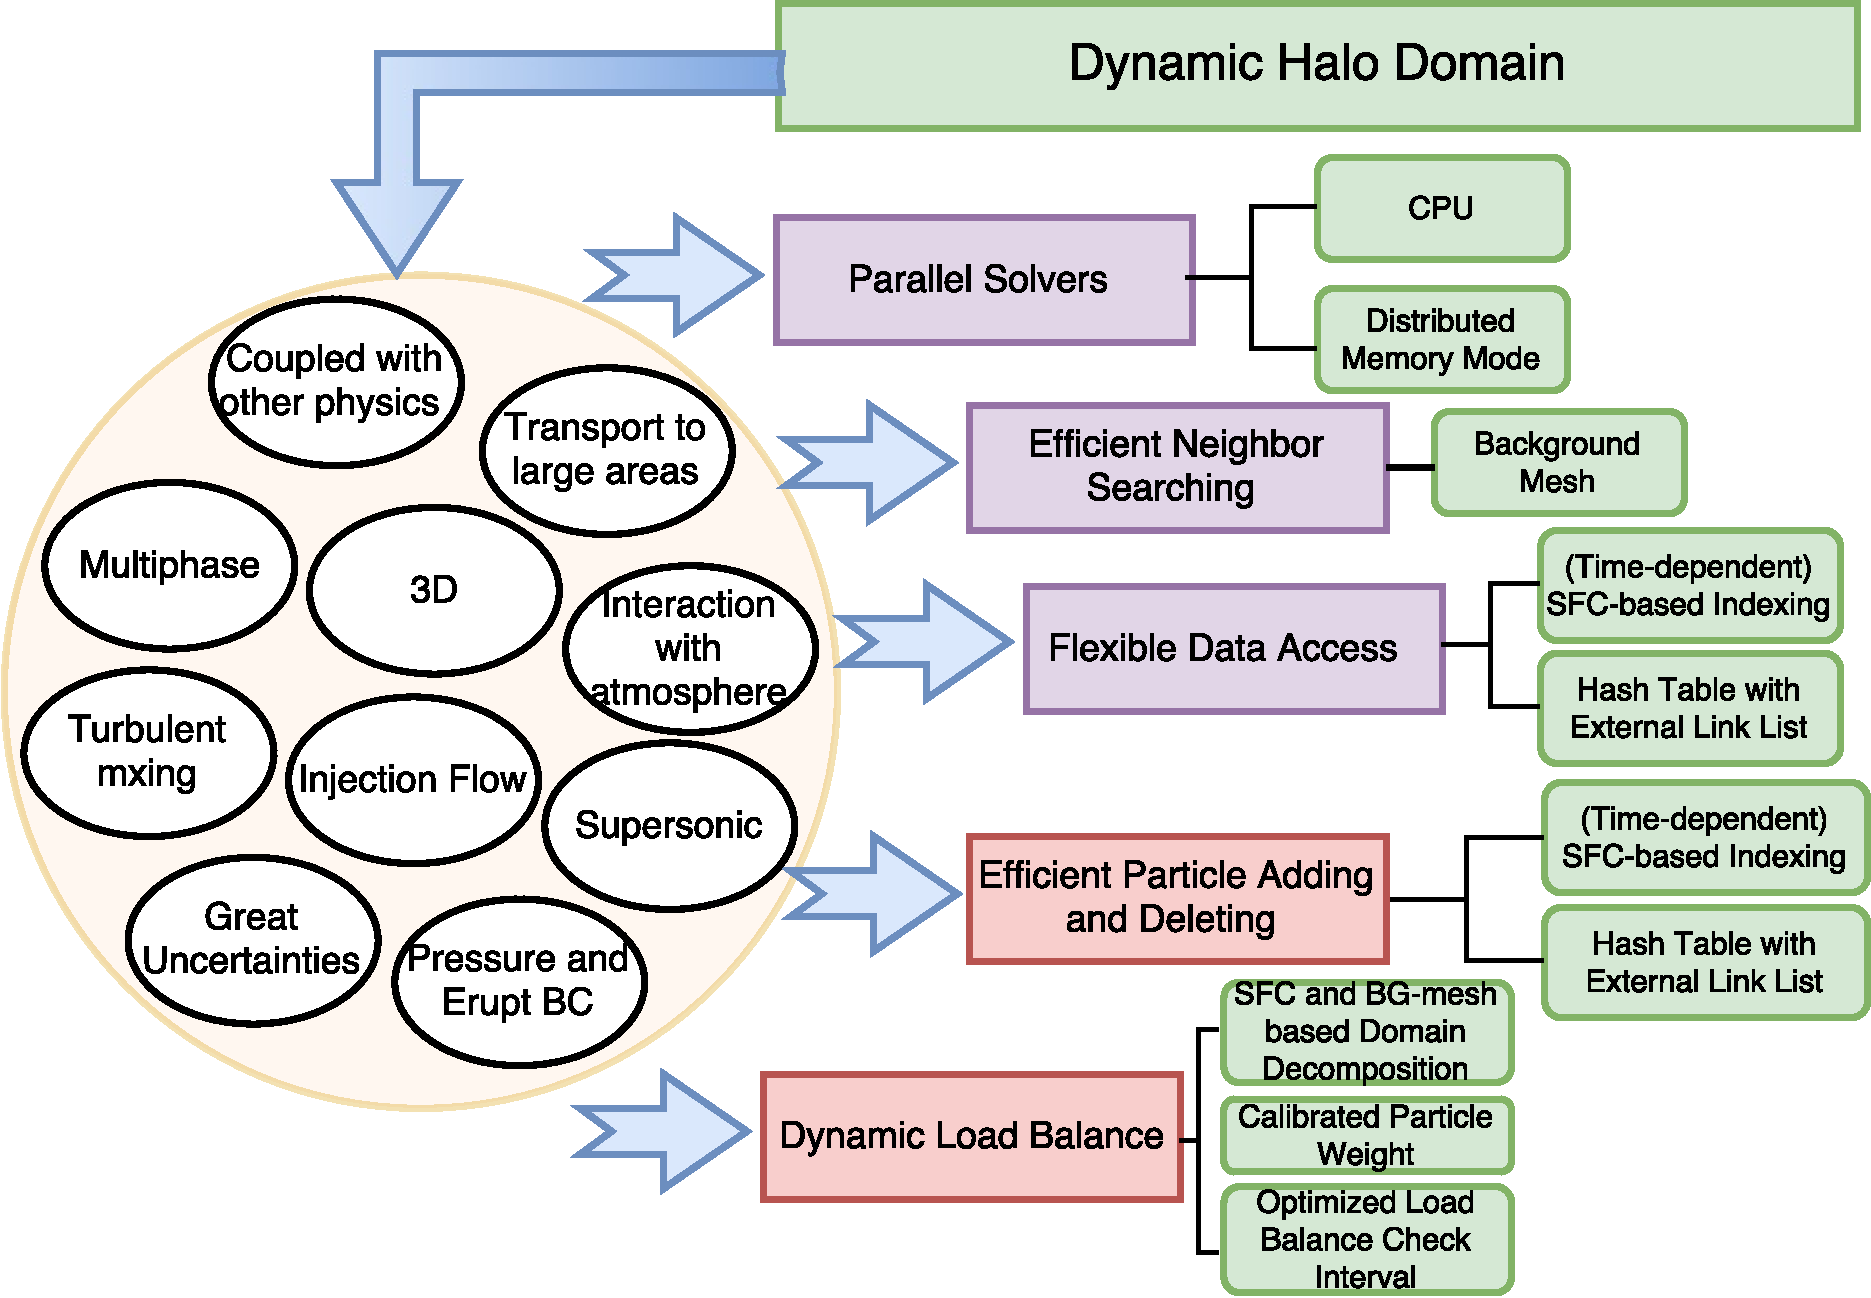
\includegraphics[scale=0.35]{Requirement_all}
%\caption{Scope of the problem}
\label{fig:Requirements}
\end{figure}
\end{frame}
%
\begin{frame}{Scalability and Computational Permormance}
\begin{minipage}{0.49\textwidth}
\begin{figure}
\center
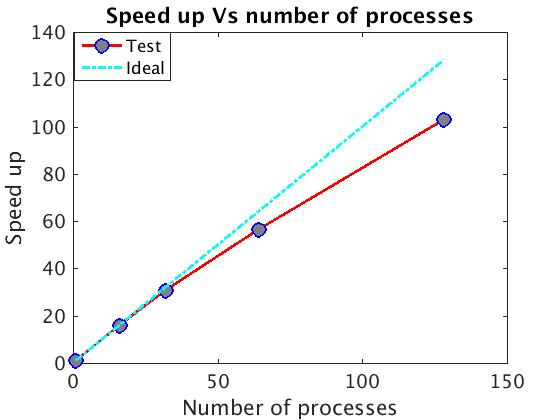
\includegraphics[width=0.75\textwidth]{../strong}
\end{figure}
\end{minipage}
%
\begin{minipage}{0.49\textwidth}
\begin{figure}
\center
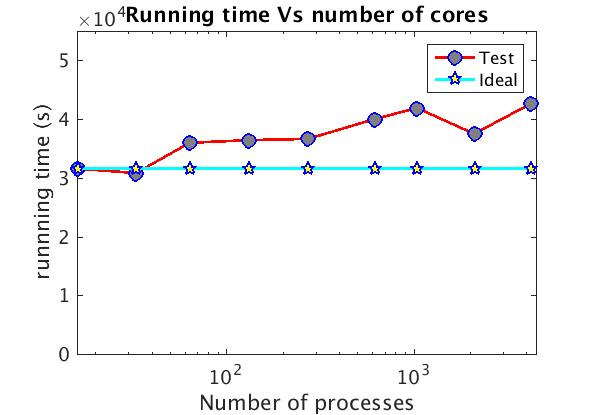
\includegraphics[width=0.75\textwidth]{../weak_scale}
\end{figure}
\end{minipage}
%
%\begin{figure}
%\center
%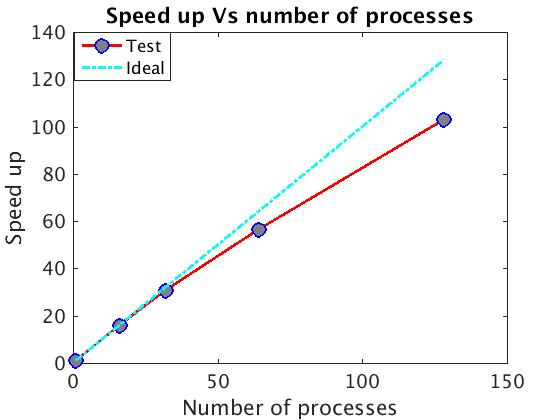
\includegraphics[width=0.35\textwidth]{../strong}
%\hfill
%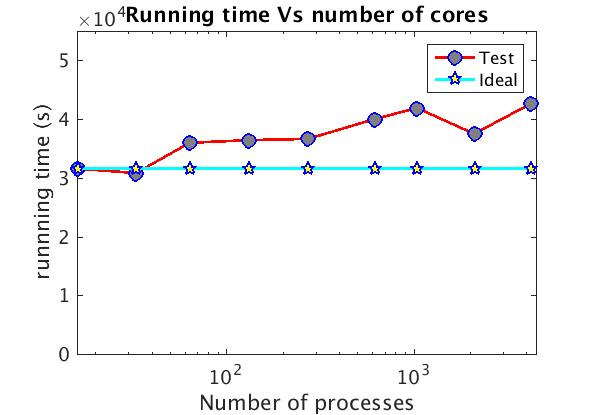
\includegraphics[width=0.35\textwidth]{../weak_scale}
%\caption{Strong scalability and weak scalability.}
%\label{fig:scalability}
%\end{figure}
%
\begin{minipage}{0.49\textwidth}
\begin{figure}
\center
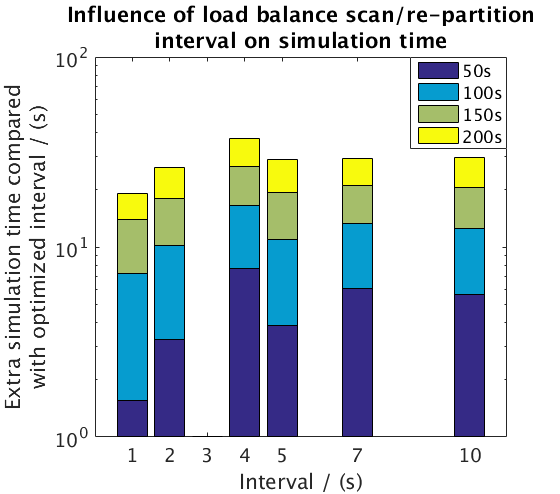
\includegraphics[width=0.75\textwidth]{int_bar}
\end{figure}
\end{minipage}
%
\begin{minipage}{0.49\textwidth}
\begin{figure}
\center
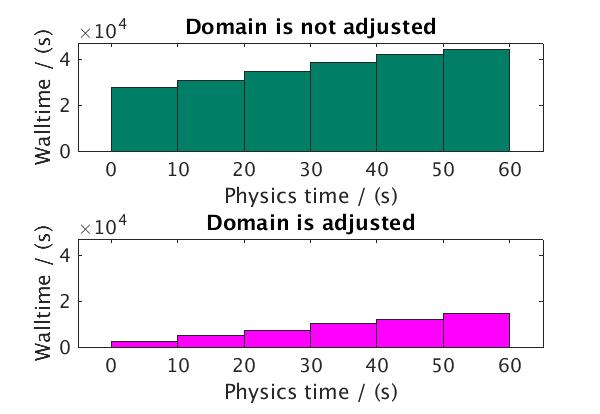
\includegraphics[width=0.75\textwidth]{../adj_vs_no}
\end{figure}
\end{minipage}
%\begin{figure}
%\flushleft
%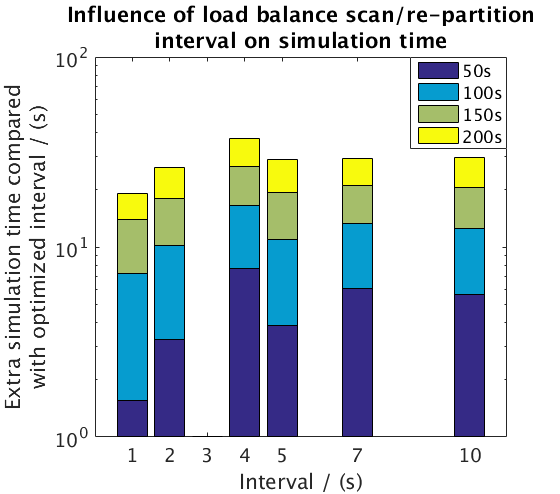
\includegraphics[width=0.35\textwidth]{int_bar}
%\hfill
%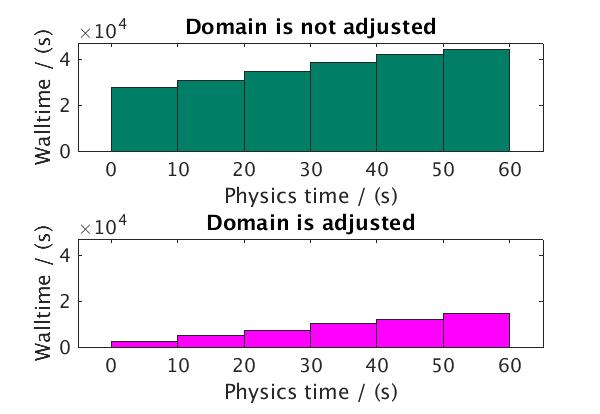
\includegraphics[width=0.35\textwidth]{../adj_vs_no}
%\caption{Effect of optimized load balance check interval and dynamic halo domain.}
%\label{fig:2cases_efficiency}
%\end{figure}
%
\end{frame}
%----------------------------------------------------------------------------
\section*{Summary}
\begin{frame}{Summary}
  \begin{itemize}
  \item
	We present an initial effort and results towards developing a first principle based plume model with comprehensive physics, adopting proper numerical tools and high performance computing.
  \item
    More advanced numerical techniques, such as adaptive particle size, Godunov-SPH, semi-explicit time advancing scheme and better data management strategies and algorithms are on our list to exploit in the future.
  \end{itemize}
\end{frame}

\begin{frame}{}
\center
\Huge{
Thank you! \\
Questions are welcome.
}

\center
zhixuanc@buffalo.edu
\end{frame}

%% All of the following is optional and typically not needed. 
%\appendix
%\section<presentation>*{\appendixname}
%\subsection<presentation>*{For Further Reading}
%
%\begin{frame}[allowframebreaks]
%  \frametitle<presentation>{For Further Reading}
%    
%  \begin{thebibliography}{10}
%    
%  \beamertemplatebookbibitems
%  % Start with overview books.
%
%  \bibitem{Author1990}
%    A.~Author.
%    \newblock {\em Handbook of Everything}.
%    \newblock Some Press, 1990.
% 
%    
%  \beamertemplatearticlebibitems
%  % Followed by interesting articles. Keep the list short. 
%
%  \bibitem{Someone2000}
%    S.~Someone.
%    \newblock On this and that.
%    \newblock {\em Journal of This and That}, 2(1):50--100,
%    2000.
%  \end{thebibliography}
%\end{frame}

\end{document}


